\documentclass[12pt,a4paper]{article}
\usepackage{amsmath, amssymb, amsthm}
\usepackage[utf8]{inputenc}
\usepackage[T1]{fontenc}
\usepackage{geometry}
\usepackage{tikz}
\usepackage{tikz-3dplot}
\usetikzlibrary{arrows.meta, calc, patterns, decorations.pathmorphing, shapes.geometric}
\geometry{margin=2.5cm}

\newtheorem{definition}{Definition}
\newtheorem{theorem}{Theorem}
\newtheorem{example}{Example}
\newtheorem{remark}{Remark}

\title{Infinitesimal Calculus 2 --- Lecture 3 (15.03.2026)\\
\large Limits of Multivariable Functions (cont.) \& Topology of $\mathbb{R}^n$}
\date{}

\begin{document}
\maketitle

%----------------------------------------------------------
\section*{Limits of Multivariable Functions (continued)}
%----------------------------------------------------------

\subsection*{$\varepsilon$-$\delta$ Definition}

\[
  \lim_{\bar{x}\to\bar{a}} f(\bar{x}) = L
\]

$\forall\varepsilon>0$, $\exists\,\delta = \delta(\varepsilon)>0$ such that:
\[
  0 < \|\bar{x}-\bar{a}\| < \delta \;\Longrightarrow\; |f(\bar{x})-L| < \varepsilon,
\]
where $d(\bar{x},\bar{a}) = \sqrt{(x_1-a_1)^2+\cdots+(x_n-a_n)^2}$.

\bigskip

\begin{example}[DNE by two paths]
\[
  \lim_{(x,y)\to(0,0)} \frac{xy}{x^2+y^2}
\]

\begin{center}
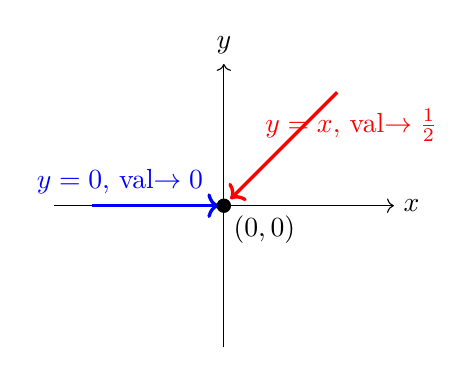
\begin{tikzpicture}[scale=1.2]
  % axes
  \draw[->] (-1.8,0) -- (1.8,0) node[right] {$x$};
  \draw[->] (0,-1.5) -- (0,1.5) node[above] {$y$};
  % path y=0 (x-axis)
  \draw[blue, very thick, ->] (-1.4,0) -- (-0.05,0);
  \node[blue] at (-1.1,0.25) {$y=0$, val$\to 0$};
  % path y=x
  \draw[red, very thick, ->] (1.2,1.2) -- (0.07,0.07);
  \node[red] at (1.35,0.85) {$y=x$, val$\to\frac{1}{2}$};
  % origin
  \filldraw (0,0) circle (2pt) node[below right] {$(0,0)$};
\end{tikzpicture}
\end{center}

\begin{itemize}
  \item Along $y=0$: $\dfrac{x\cdot 0}{x^2+0}=0\to 0$.
  \item Along $y=x$: $\dfrac{x\cdot x}{x^2+x^2}=\dfrac{1}{2}$.
\end{itemize}
Two different values $\Rightarrow$ \textbf{limit does not exist}.
\end{example}

\begin{example}[Polar coordinates --- limit $= 0$]
\[
  \lim_{(x,y)\to(0,0)} \frac{xy^2}{x^2+y^2} = 0
\]
Substituting $x=\rho\cos\theta$, $y=\rho\sin\theta$:
\[
  \frac{xy^2}{x^2+y^2} = \rho\cos\theta\sin^2\theta \xrightarrow{\rho\to 0} 0
  \quad \text{(Squeeze: }|xy^2/(x^2+y^2)|\le|y|\to 0\text{)}.
\]
\end{example}

\begin{example}[DNE by two paths --- tricky case]
\[
  \lim_{(x,y)\to(0,0)} \frac{xy^2}{x^2+y^4}
\]

\begin{center}
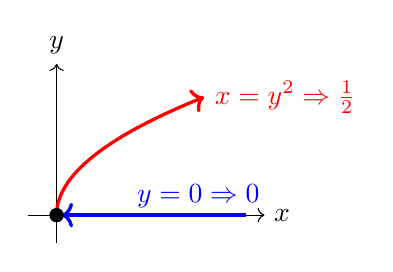
\begin{tikzpicture}[scale=1.2]
  \draw[->] (-0.3,0) -- (2.2,0) node[right] {$x$};
  \draw[->] (0,-0.3) -- (0,1.6) node[above] {$y$};
  % path y=0
  \draw[blue, very thick, ->] (2.0,0) -- (0.05,0);
  \node[blue] at (1.5,0.2) {$y=0 \Rightarrow 0$};
  % path x=y^2 (parabola)
  \draw[red, very thick, domain=0:1.25, samples=60, ->]
    plot (\x*\x, \x) node[right] {$x=y^2 \Rightarrow\frac{1}{2}$};
  \filldraw (0,0) circle (2pt);
\end{tikzpicture}
\end{center}

\begin{itemize}
  \item Along $y=0$: limit $= 0$.
  \item Along $x=y^2$: $\dfrac{y^2\cdot y^2}{y^4+y^4}=\dfrac{1}{2}$.
\end{itemize}
\textbf{The limit does not exist.}
\end{example}

\begin{example}[Polar with bounding trick --- limit $= 0$]
\[
  \lim_{(x,y)\to(0,0)} \frac{x^2 y^2(x^2+y^2)}{x^4+y^4}
\]
Converting to polar:
\[
  = \lim_{\rho\to 0}\rho^2\cdot
    \frac{\cos^2\theta\sin^2\theta}{\cos^4\theta+\sin^4\theta}.
\]
\textbf{Key bound}: Using $(a+b)^2 = a^2+2ab+b^2$ with $a=\cos^2\theta$, $b=\sin^2\theta$:
\[
  \cos^4\theta+\sin^4\theta = 1 - 2\cos^2\theta\sin^2\theta
  = 1-\tfrac{1}{2}\sin^2 2\theta \;\ge\; \frac{1}{2}.
\]
Hence $0\le\dfrac{\cos^2\theta\sin^2\theta}{\cos^4\theta+\sin^4\theta}\le 2$,
and by Squeeze: $\rho^2\cdot(\text{bounded})\to \mathbf{0}$.
\end{example}

\begin{example}[Not defined on a path $\Rightarrow$ limit DNE]
\[
  \lim_{(x,y)\to(0,0)} \frac{\sin(x-y)}{x-y}
\]

\begin{center}
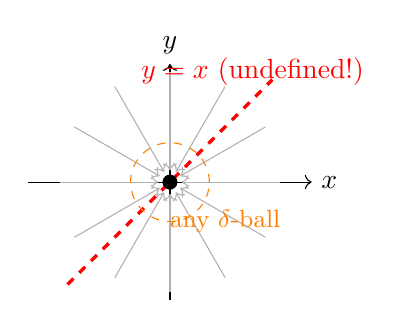
\begin{tikzpicture}[scale=1.0]
  \draw[->] (-1.8,0) -- (1.8,0) node[right] {$x$};
  \draw[->] (0,-1.5) -- (0,1.5) node[above] {$y$};
  % many approach paths (flower)
  \foreach \angle in {0,30,60,90,120,150,180,210,240,270,300,330}{
    \draw[gray!60, ->] (\angle:1.4) -- (\angle:0.15);
  }
  % the forbidden path y=x
  \draw[red, very thick, dashed] (-1.3,-1.3) -- (1.3,1.3);
  \node[red] at (1.05,1.4) {$y=x$ (undefined!)};
  \filldraw (0,0) circle (2.5pt);
  % dashed circle around origin
  \draw[orange, dashed] (0,0) circle (0.5);
  \node[orange] at (0.7,-0.5) {\small any $\delta$-ball};
\end{tikzpicture}
\end{center}

The path $y=x$ passes through $(0,0)$ and the function is undefined there ($x-y=0$).
No punctured neighbourhood of $(0,0)$ exists in which $f$ is defined everywhere.
Hence \textbf{the limit cannot be discussed / does not exist}.

Note: $\lim_{z\to 0}\dfrac{\sin z}{z}=1$, but $z=x-y=0$ on the entire line $y=x$.
\end{example}

%----------------------------------------------------------
\section*{Continuity of Multivariable Functions}
%----------------------------------------------------------

\begin{definition}[Continuity at a point]
$f(\bar{x})$ is \textbf{continuous} at $\bar{a}$ if:
\[
  \lim_{\bar{x}\to\bar{a}} f(\bar{x}) = f(\bar{a}).
\]
For two variables: $\displaystyle\lim_{(x,y)\to(x_0,y_0)} f(x,y) = f(x_0,y_0)$.
\end{definition}

The \textbf{increment} of $f$ at $(x_0,y_0)$:
\[
  \Delta f(x_0,y_0) = f(x_0+\Delta x,\, y_0+\Delta y) - f(x_0,y_0).
\]
Continuity $\iff$ $\displaystyle\lim_{(x,y)\to(x_0,y_0)}\Delta f(x_0,y_0) = 0$.

%----------------------------------------------------------
\section*{Topology of Euclidean Space $\mathbb{R}^n$}
%----------------------------------------------------------

\begin{definition}[Open ball]
$B(\bar{a},r) = \{\bar{x} : \|\bar{x}-\bar{a}\| < r\}$ is the \textbf{open ball}
of radius $r$ centred at $\bar{a}$.
\end{definition}

\begin{center}
\begin{tikzpicture}[scale=1.1]
  \draw[->] (-0.5,0) -- (3.5,0) node[right] {$x$};
  \draw[->] (0,-0.5) -- (0,2.5) node[above] {$y$};
  % open ball
  \draw[green!70!black, dashed, thick] (2,1.2) circle (0.7);
  \node[green!70!black] at (2.9,1.9) {$B(\bar{a},r)$};
  \filldraw[green!70!black] (2,1.2) circle (2pt) node[below right] {$\bar{a}$};
  % radius label
  \draw[green!70!black] (2,1.2) -- (2.7,1.2) node[midway, above] {\small $r$};
\end{tikzpicture}
\end{center}

\begin{definition}[Interior point (Def.\ 2)]
$\bar{a}$ is an \textbf{interior point} of $E$ if $\exists\,r>0$ such that $B(\bar{a},r)\subseteq E$.
\end{definition}

\begin{definition}[Exterior point (Def.\ 3)]
$\bar{a}$ is an \textbf{exterior point} of $E$ if $\exists\,r>0$ such that $B(\bar{a},r)\cap E=\emptyset$.
\end{definition}

\begin{definition}[Boundary point (Def.\ 4)]
$\bar{a}$ is a \textbf{boundary point} of $E$ if every $B(\bar{a},r)$ meets both $E$ and $\mathbb{R}^n\setminus E$.
\end{definition}

\begin{center}
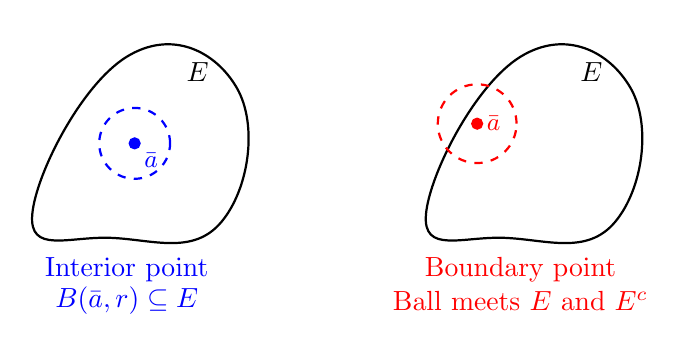
\begin{tikzpicture}[scale=1.0]
  %--- Interior point ---
  \begin{scope}[xshift=0cm]
    % region E
    \draw[thick] plot[smooth cycle, tension=0.8]
      coordinates {(-1.2,-0.8)(0,1.2)(1.4,0.8)(1.2,-0.9)(-0.2,-1.1)};
    \node at (0.9,1.0) {$E$};
    % interior ball
    \draw[blue, dashed, thick] (0.1,0.1) circle (0.45);
    \filldraw[blue] (0.1,0.1) circle (2pt) node[below right] {\small $\bar{a}$};
    \node[blue] at (0,-1.5) {Interior point};
    \node[blue] at (0,-1.9) {$B(\bar{a},r)\subseteq E$};
  \end{scope}
  %--- Boundary point ---
  \begin{scope}[xshift=5cm]
    \draw[thick] plot[smooth cycle, tension=0.8]
      coordinates {(-1.2,-0.8)(0,1.2)(1.4,0.8)(1.2,-0.9)(-0.2,-1.1)};
    \node at (0.9,1.0) {$E$};
    % boundary ball straddles the edge
    \draw[red, dashed, thick] (-0.55,0.35) circle (0.5);
    \filldraw[red] (-0.55,0.35) circle (2pt) node[right] {\small $\bar{a}$};
    \node[red] at (0,-1.5) {Boundary point};
    \node[red] at (0,-1.9) {Ball meets $E$ and $E^c$};
  \end{scope}
\end{tikzpicture}
\end{center}

\begin{definition}[Interior, Exterior, Boundary]
\[
  \operatorname{Int} E,\qquad \operatorname{Ext} E,\qquad \partial E.
\]
\end{definition}

\begin{definition}[Open set (Def.\ 8)]
$E$ is \textbf{open} $\iff$ $E = \operatorname{Int} E$ (every point is interior).
\end{definition}

\begin{definition}[Closed set (Def.\ 9)]
$E$ is \textbf{closed} $\iff$ $\partial E\subseteq E$.
\textit{Remark}: $E$ closed $\iff$ $\mathbb{R}^n\setminus E$ is open.
\end{definition}

\begin{definition}[Bounded (Def.\ 10) \& Compact (Def.\ 11)]
$E$ is \textbf{bounded} if $E\subseteq B(\bar{a},r)$ for some ball.
$E$ is \textbf{compact} if it is \emph{closed and bounded}.
\end{definition}

\begin{center}
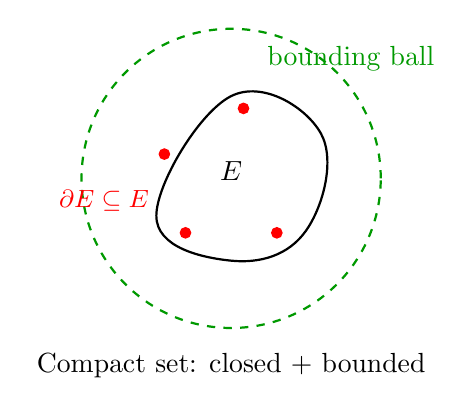
\begin{tikzpicture}[scale=0.95]
  % large circle = bounding ball
  \draw[green!60!black, thick, dashed] (0,0) circle (2.0);
  \node[green!60!black] at (1.6,1.6) {bounding ball};
  % compact set inside
  \draw[thick] plot[smooth cycle, tension=0.7]
    coordinates {(-1,-0.5)(0,1.1)(1.2,0.6)(1,-0.7)(0,-1.1)};
  \node at (0,0.1) {$E$};
  \node at (0,-2.5) {Compact set: closed $+$ bounded};
  % boundary points marked
  \foreach \angle in {80,160,230,310}{
    \filldraw[red] (\angle:0.95) circle (2pt);
  }
  \node[red] at (-1.7,-0.3) {\small$\partial E\subseteq E$};
\end{tikzpicture}
\end{center}

\subsection*{Weierstrass Theorems}

\begin{theorem}[Weierstrass 1]
A function $f(\bar{x})$ continuous on a compact set is \emph{bounded} on it.
\end{theorem}

\begin{theorem}[Weierstrass 2]
If $f(\bar{x})$ is continuous on compact $E$, then $f$ attains
$M=\sup_E f(\bar{x})$ and $m=\inf_E f(\bar{x})$.
\end{theorem}

\end{document}
